%
% File acl2020.tex
%
%% Based on the style files for ACL 2020, which were
%% Based on the style files for ACL 2018, NAACL 2018/19, which were
%% Based on the style files for ACL-2015, with some improvements
%%  taken from the NAACL-2016 style
%% Based on the style files for ACL-2014, which were, in turn,
%% based on ACL-2013, ACL-2012, ACL-2011, ACL-2010, ACL-IJCNLP-2009,
%% EACL-2009, IJCNLP-2008...
%% Based on the style files for EACL 2006 by 
%%e.agirre@ehu.es or Sergi.Balari@uab.es
%% and that of ACL 08 by Joakim Nivre and Noah Smith

\documentclass[11pt,a4paper]{article}
\usepackage[hyperref]{acl2020}
\usepackage{times}
\usepackage{graphicx}
\usepackage{tabularx}
\graphicspath{ {./images/} }
\usepackage{latexsym}
\renewcommand{\UrlFont}{\ttfamily\small}
\DeclareCaptionLabelFormat{suppl}{#1~S#2}%

% This is not strictly necessary, and may be commented out,
% but it will improve the layout of the manuscript,
% and will typically save some space.
\usepackage{microtype}

\aclfinalcopy
%\def\aclpaperid{***} %  Enter the acl Paper ID here

%\setlength\titlebox{5cm}
% You can expand the titlebox if you need extra space
% to show all the authors. Please do not make the titlebox
% smaller than 5cm (the original size); we will check this
% in the camera-ready version and ask you to change it back.

\newcommand\BibTeX{B\textsc{ib}\TeX}

\title{Measuring Difficulty: Conceptual Foreknowledge Requirements and Coherence in Scientific Literature
}

\author{Caralyn Reisle \\
  University of British Columbia \\
  Genome Sciences Centre \\
  \texttt{creisle@bcgsc.ca} \\\And
  Oloff Biermann \\
  University of British Columbia \\
  Department of Computer Science \\
  \texttt{ocbier@cs.ubc.ca} \\}

\date{}

\begin{document}
\maketitle
\begin{abstract}
In the last two decades, the reading burden on researchers has increased significantly. However, asssistive tools and underlying methods for navigating the vast array of published material have not kept up with this growth. We present both a global LDA-based coherence scoring method and a supervised concept extraction framework. Together, these offer a promising solution for assessing readability and conceptual foreknowledge requirements which is applicable in supporting tools for researchers, most notably recommender systems. We evaluated our approach on large data sets of scientific literature and contrast our coherence scoring method with traditional "shallow" readability scoring. In addition to our results, we provide a design for an open-source tool to record data on users as they browse papers. 
\end{abstract}

\section{Introduction}

Most work on readability or measuring text difficulty has focused on accessibility to the general population which assumes a low reading level. However an analogous problem exists within research itself. As the domain of knowledge increases, so does the burden on the researchers (Figure \ref{fig:articles-published}). Increasingly scientific literature requires domain-specific knowledge and vernacular which is a barrier to entry \cite{Plaven-Sigray2017-xb}.

\begin{figure}
    \centering
    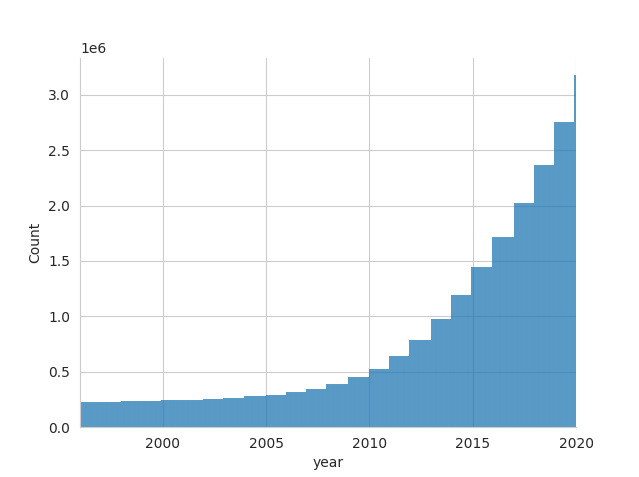
\includegraphics[width=8cm]{images/cumulative-articles-published.png}
    \caption{Cumulative Number of Articles published by Year in the Open Access PMC corpus}
    \label{fig:articles-published}
\end{figure}

Sentence complexity has historically been used as the sole metric for predicting comprehension difficulty. Most readability scores depend heavily on word and sentence length which are not always a good measure of simplicity, particularly in scientific or health-related literature \cite{Kauchak2017-ox}. We applied traditional scoring to a subset of the articles available from PubMed central full text articles open data set.

While the traditional metrics for readability are relatively easy to calculate and computationally inexpensive, they are overly simplistic and do not provide an accurate measure of text coherence \cite{Balyan2020-zr}. They are shallow and do not adequately capture semantic aspects of discourse beyond superficial syntactic features. Thus, applying readability techniques to scientific literature would not give the most useful result. By contrast, machine learning based methods employ a deeper representation of language features to assess coherence more accurately. 

\section{Related Work}

\paragraph{Readability and coherence:}
Previous work in this area has leveraged rhetorical structure theory (RST) based approaches for coherence classification \cite{Guz2020-ap}. Other work has used techniques such as latent semantic analysis (LSA) and latent dirichlet allocation (LDA) to assess coherence at the sentence-to-sentence, sentence-to-paragraph, and paragraph-to-paragraph levels. This includes tools such as Coh-metrix \cite{Graesser2004-lg} and TAACO 2.0 \cite{Crossley2019-ln}. TAACO 2.0 is a tool which assesses multiple factors to give a comprehensive assessment of cohesion, a key factor impacting coherence. In adult readers, local cohesion is negatively correlated with coherence. However, the opposite is true for global cohesion features, which show a strong correlation with coherence \cite{Crossley2019-ln}.

\paragraph{Concept Extraction:}
Both sentence complexity and coherence deal with the composition of the article but ignore the conceptual content. Science is built on an ever growing baseline of concepts and vernacular. Here we aim to measure the number of concepts the reader is required to know in order to effectively read a given scientific article. The number of new concepts a reader must cover will contribute to the overall difficulty. This is supported by previous work which demonstrated that term (word) familiarly had a greater impact on users' reading difficulty than word length \cite{Leroy2014-ft}. Concept extraction through named entity recognition is a popular area of research in natural language processing. Previous work has been done on extracting and classifying concepts from the titles of scientific articles \cite{Krishnan2017-eo}. This was used as a proxy for measuring their major contributions. Other work in this area has focused on general scientific concepts which are not domain specific \cite{Brack2020-id}. 

The long term goal of this project is a recommender system for researchers that will optimize learning a new field by recommending papers that are not overly complex and match the researchers knowledge level in the field. This will involve the assessment of three metrics to represent the overall difficulty of comprehension of a particular article: sentence syntactic complexity (readability); coherence (flow/cohesion); and foreknowledge (concept) requirements of scientific literature. Since the primary target of work in this area has been generally low reading levels for consumption by the general public, the data sets these techniques are applied to are vastly different from the PMC corpus of scientific articles. 



\section{Contribution}
\label{sec:contribution}
This project makes contributions in five main areas as follows:
\begin{enumerate}
\item Evaluation of readability on papers in the PMC corpus using traditional scoring methods
\item Evaluation of LDA coherence scoring systems against traditional readability scoring when applied to scientific literature in the PMC and GCDC corpuses
\item A framework for measuring knowledge requirements through concept extraction
\item The design for an open source browser extension which collects data on user behaviour as they browse scientific literature
\end{enumerate}

\section{Data sets}
The following data sets were used
\begin{enumerate}
    \item \textbf{PMC}: Pubmed Central biomedical and life sciences journal articles, full-text open access data set.
    \item \textbf{OA-STM}: Corpus of Open Access articles from multiple fields in Science, Technology, and Medicine (110 articles)
    \item \textbf{GCDC}: Grammarly Corpus of Discourse Coherence
    \item \textbf{Entrez API:} API which can be used to fetch article metadata for PMC/Pubmed articles
    \item \textbf{PubMed Knowledge Graph:} A disambiguated collection of author and institution metadata for articles from Semantic Scholar, PubMed, and other large corpora
\end{enumerate}

The PMC data set was the primary data set used for analysis, the others were used in evaluating the below techniques or replicating existing methods to exclude system bias prior to applying them to the PMC data set. 
See the appendix for corpus access information.


\section{Methods and Implementation}

\paragraph{Metadata Collection:}
Metadata regarding the PMC corpus was collected from two sources: the Entrez API \cite{Sayers2010-zl}; and the PubMed Knowledge Graph \cite{Xu2020-hq}. The Entrez API was used to collect information regarding the written language of the article as well as type classifications such as 'Review'. Articles not written in English articles were excluded from analysis. The PubMed Knowledge Graph was used to collect author and author affiliation data. The first affiliation of the first author of each article was determined. This was then parsed to determine the country the affiliated institute resides in (Figure \ref{fig:pmc-by-region}).

\begin{figure}
    \centering
    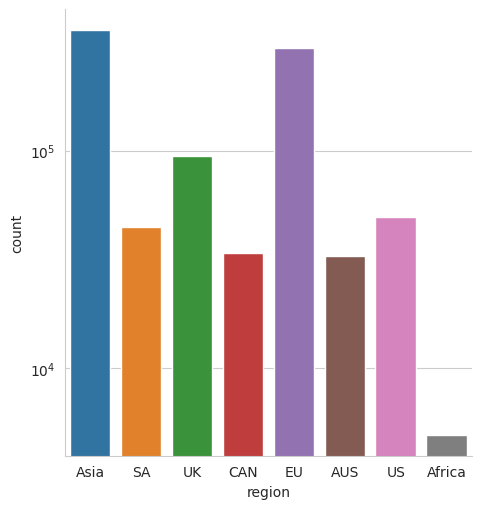
\includegraphics[width=8cm]{images/pmc.country.histogram.png}
    \caption{Number of Publications by Region of the Location of the First Author First Affiliation Institution. Regions are divided into: Australia and New Zealand (AUS); South America (SA); Asia; United Kingdom (UK); United States (US); Canada (CAN); Europe, excluding UK (EU); and Africa}
    \label{fig:pmc-by-region}
\end{figure}

Using the above metadata, the remaining articles were divided into two groups based on our assumptions about readability:
\begin{enumerate}
\item \textbf{First Author English Affiliation Group (FAEA)}: The first affiliation of the first author of the article is based in an English speaking country (US, UK, Canada, Australia).
\item \textbf{First Author Non-English Affiliation Group (FANA)}: The first affiliation of the first author of the article is not based in an English speaking country
\end{enumerate}

We made the assumption that papers in the English Affiliation (FAEA) group are more readable and should give a higher coherence score, on average. It should be noted that in the interest of computational efficiency, we performed the calculations and modelling described in the subsequent subsections first before performing splitting. Following splitting, we performed analysis on the results (Figure \ref{fig:system-overview}).

\begin{center}
\begin{figure*}
    \centering
    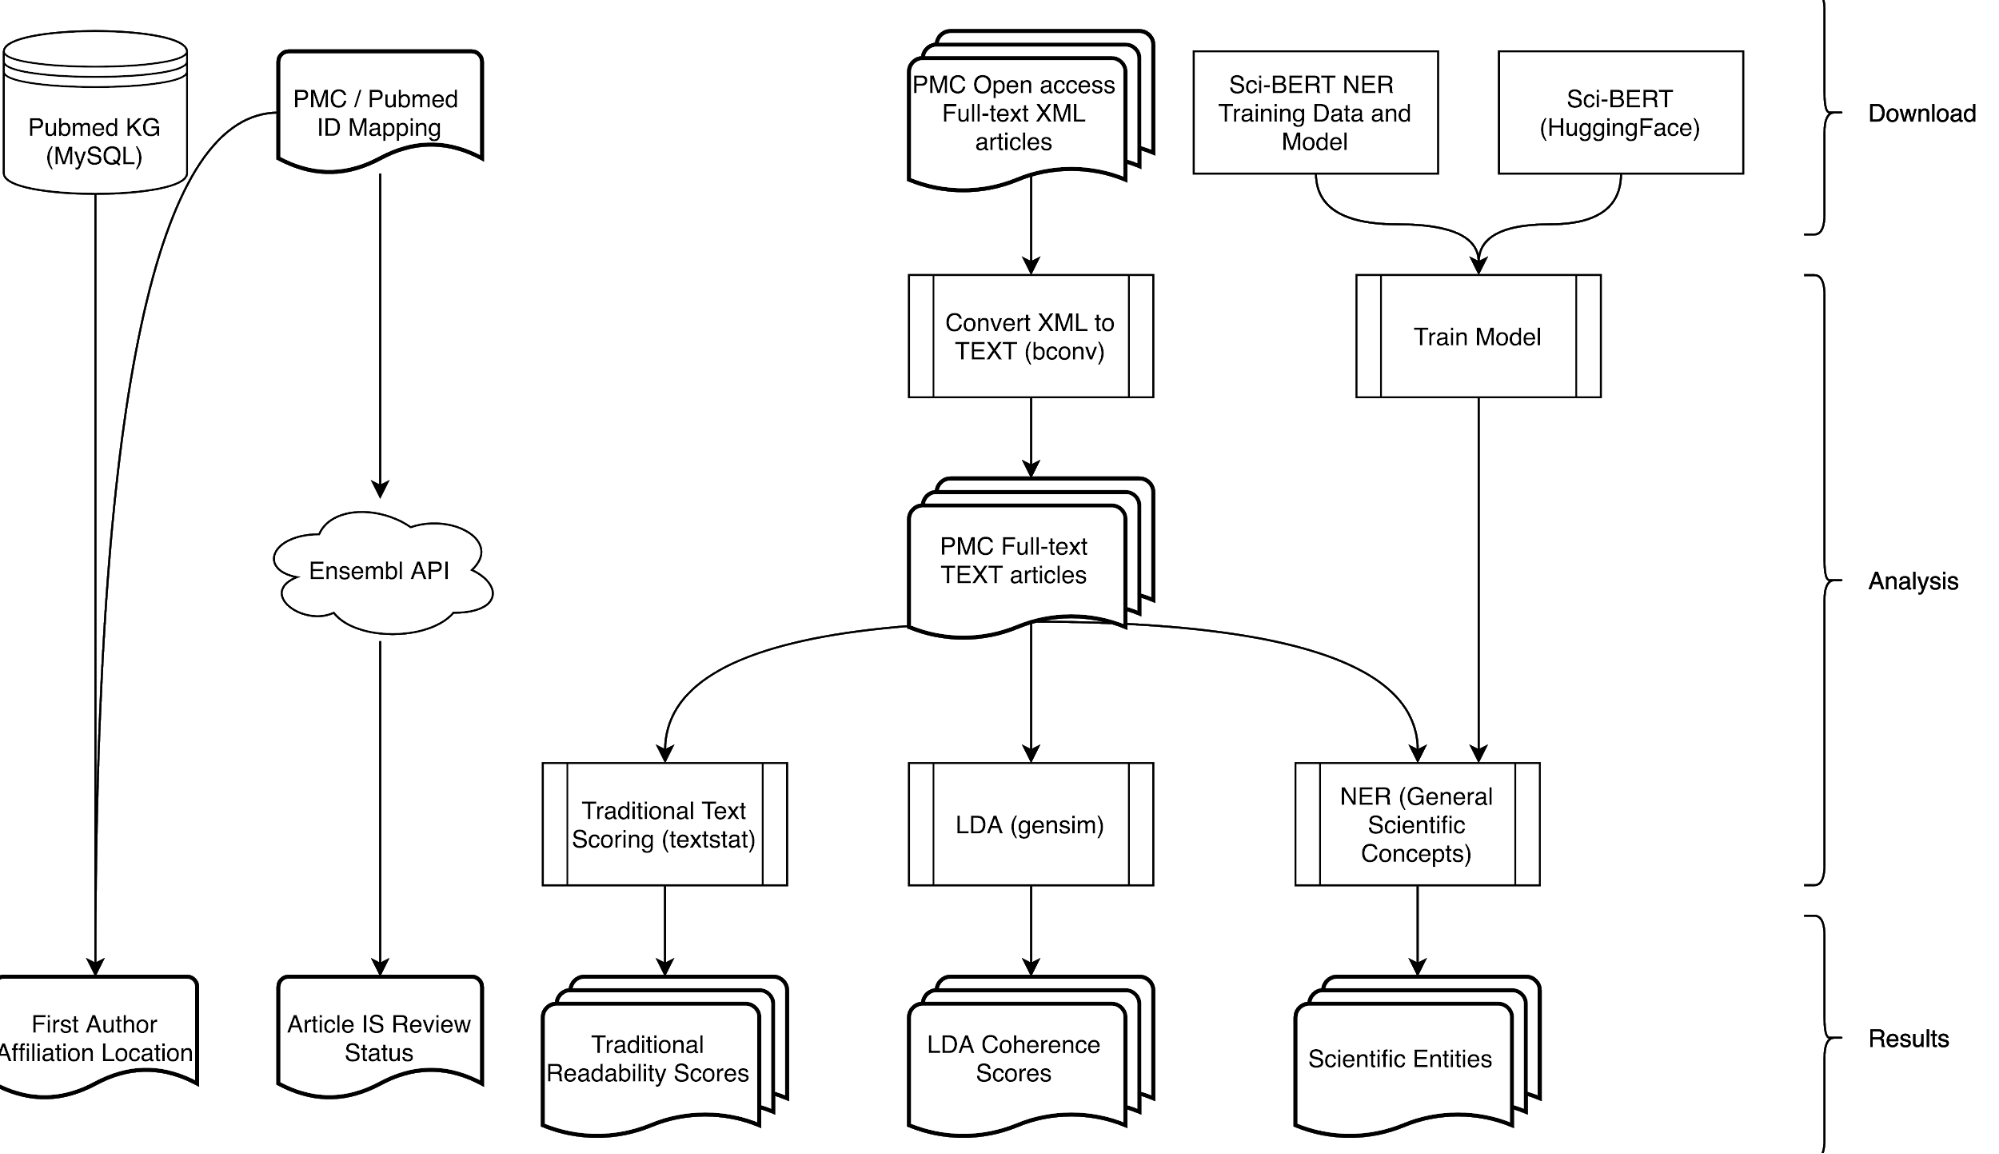
\includegraphics[width=15cm]{images/system-architecture.png}
    \caption{System architecture overview. Snakemake (\url{https://snakemake.readthedocs.io/en/stable/index.html}) workflows were written to compute the pipelines above in parallel.}
    \label{fig:system-overview}
\end{figure*}
\end{center}

\paragraph{Pre-processing:}
We pre-processed each article to convert from NXML to text using the Python package bconv (\url{https://pypi.org/project/bconv}). The processed data included all articles with length \(1000 < m < 100,000\), where m is the number of characters (Figure \ref{fig:text-length}). 

\begin{figure}
    \centering
    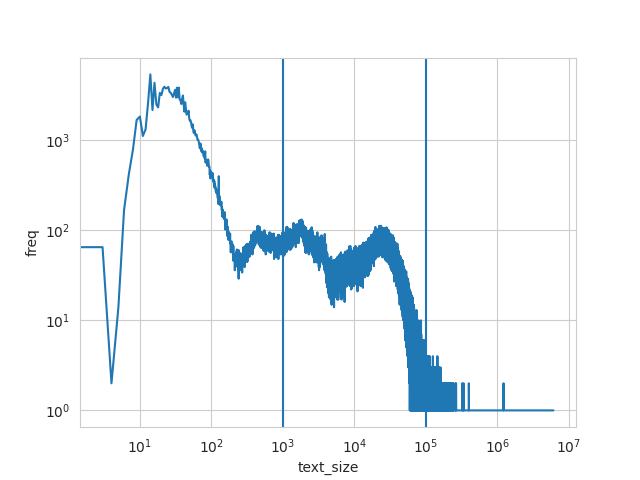
\includegraphics[width=8cm]{images/pmc.text_size.lineplot.png}
    \caption{Text Length in characters post-text conversion with bconv of articles in the PMC corpus. Vertical lines represent chosen thresholds of 1000 and 100,000 characters.}
    \label{fig:text-length}
\end{figure}

The lower threshold was chosen as \(m < 1000\) characters often represents incomplete articles where the full text nXML file contained only the article title and links. Additionally the LDA coherence scoring was not reliable with shorter text sizes A The upper threshold was chosen to limit the data set to the proportion of articles with comparable frequency. This was done to attempt to mitigate the influence of text length on the results.

We applied five traditional readability scoring methods on the PMC corpus using the Python package textstat (\url{https://pypi.org/project/textstat}). Given the size of the data set, we performed calculations in parallel using a batched approach. We specifically considered the following metrics: The Flesch-Kincaid Grade Level; Flesch Reading Ease; Gunning FOG Index; Automated Readability Index; and Coleman-Liau Index.

\paragraph{LDA Coherence:}
To measure coherence, we used an LDA model constructed with gensim (\url{https://github.com/RaRe-Technologies/gensim}) in Python. Starting with the pre-processed texts, we first removed stop words and punctuation. We then performed tokenization and formed a set bigrams. Given these bigrams, we performed lemmatization with \href{https://spacy.io/}{spaCy}. Finally, we created a dictionary with ID mappings to the lemmas. For model hyperparameters we chose moderate values of alpha=0.1 and eta= 0.9. We considered that we wish to capture the main topics within each paper and that there would be some overlap in the words occurring within each topic. 

\paragraph{}
Thus we generated coherence scores on the PMC and GCDC \cite{Lai2018-qp} data sets. As in the case of the traditional readability metrics, we used parallelization to significantly reduce the running time. Specifically, we used the multi-core LDA model provided by \href{https://github.com/RaRe-Technologies/gensim}{gensim}.

\paragraph{Concept Extraction:}

We applied the domain independent scientific concept extraction model described in Brack 2020 to the PMC dataset. Their domain independent model leverages sci-BERT \cite{Beltagy2019-vz} encodings and a supervised neural network to label concepts. The model consists of a token embedding layer which uses a concatenation of BERT embeddings and a character level convolutional neural net (CNN) based embedding. These are then encoded using bidirectional long short-term memory (LSTM) followed by a multi-layer perceptron. Finally these encodings are decoded using a conditional random field (CRF) decoder. Four concept types are labelled: Data, Material, Method and Process.
First the model was trained and evaluated as described  \cite{Brack2020-id} to ensure reproducibility of the reported results. The STM corpus articles were downloaded as well as the pre-trained sci-BERT embeddings and used to train the model. The trained model was evaluated by five-fold cross validation. Following this, the model was used to generate concept labels for articles from the PMC corpus. Post-processing using spaCy (\url{https://spacy.io}) was done on the extracted concepts to simplify comparison. Extracted concept tokens were simplified by converting words to their lemma and removing numbers as well as 'non-acronym’ stop-words. Stop Words with only capital letters which were not the sentence start were considered acronyms and not removed. The extracted concepts were used to generate clusters of articles using agglomerative hierarchical clustering with an average linkage function and a distance threshold of \( c - 1 \) where c is the total number of unique concepts extracted. \newline \newline The distance function was computed as 
\begin{equation}
d = c - \vec{x} \bullet \vec{y} 
\end{equation}
where x and y are zero vectors the size of c which represent embeddings of the extracted concepts for each article. 

\section{Results and Evaluation}

\paragraph{Readability Scoring:} Looking first at the outcome of analysis with the five traditional readability metrics, these showed no meaningful differences between English affiliation group (FAEA; n = 202,598)  and non-English affiliation group (FANA; n = 2,604,242) when considering the means (Figure \ref{fig:readability-scores}). While there was a statistically significant difference between the groups for all five metrics, this does not give a useful classification considering the scale of these metrics. Additionally, the medians of score distributions for both groups across all metrics paradoxically do not reflect this difference (Table \ref{table:scores}). In other words, the medians suggest that the FANA group is slightly more readable than FAEA. This was unexpected and bears further investigation.

\begin{center}
\begin{table*}[ht]
\centering
\caption{LDA and traditional readability metrics for first-author English affiliation (FAEA) and  first-author non-English affiliation FANA. Traditional metrics include: Flesch-Kincaid Grade Level (FKGL); Flesch Reading Ease (FRE); Gunning FOG Index (GFI); Automated Readability Index (ARI); and Coleman-Liau Index (CLI). Additionally the LDA coherence score (LDA) and the p-value for the Welch's T-test between the means of the two groups are reported (FAEA vs FANA)}
\begin{tabular}{|c | c | c | c| c | c | c |c| }
\label{table:scores}
\textbf{Measure} & \textbf{FAEA} & \textbf{Mean} & \textbf{Median} & \textbf{StdDev} & \textbf{Size} & \textbf{t} & \textbf{p-value (welch)} \\
\hline
LDA & FALSE & 4.86E-01 & 4.61E-01 & 1.69E-01 & 1.11E+06 & 48.29 & 0.00E+00 \\
 & TRUE & 5.25E-01 & 4.75E-01 & 2.06E-01 & 7.03E+04 & 48.29 & 0.00E+00 \\
ARI & FALSE & 2.28E+01 & 2.15E+01 & 1.27E+01 & 2.60E+06 & 27.15 & 3.49E-162 \\
 & TRUE & 2.32E+01 & 2.24E+01 & 5.31E+00 & 2.03E+05 & 27.15 & 3.49E-162 \\
CLI & FALSE & 1.56E+01 & 1.51E+01 & 1.18E+01 & 2.60E+06 & -37.16 & 4.83E-302 \\
 & TRUE & 1.53E+01 & 1.52E+01 & 2.19E+00 & 2.03E+05 & -37.16 & 4.83E-302 \\
FGKL & FALSE & 1.80E+01 & 1.71E+01 & 6.01E+00 & 2.60E+06 & 53.54 & 0.00E+00 \\
 & TRUE & 1.85E+01 & 1.79E+01 & 4.06E+00 & 2.03E+05 & 53.54 & 0.00E+00 \\
FRE & FALSE & 2.60E+01 & 2.88E+01 & 2.28E+01 & 2.60E+06 & -23.82 & 2.68E-125 \\
 & TRUE & 2.52E+01 & 2.67E+01 & 1.41E+01 & 2.03E+05 & -23.82 & 2.68E-125 \\
GFI & FALSE & 1.68E+01 & 1.60E+01 & 5.49E+00 & 2.60E+06 & 68.66 & 0.00E+00 \\
 & TRUE & 1.74E+01 & 1.68E+01 & 3.88E+00 & 2.03E+05 & 68.66 & 0.00E+00 \\
\end{tabular}
\end{table*}
\end{center}

\begin{figure}
    \centering
    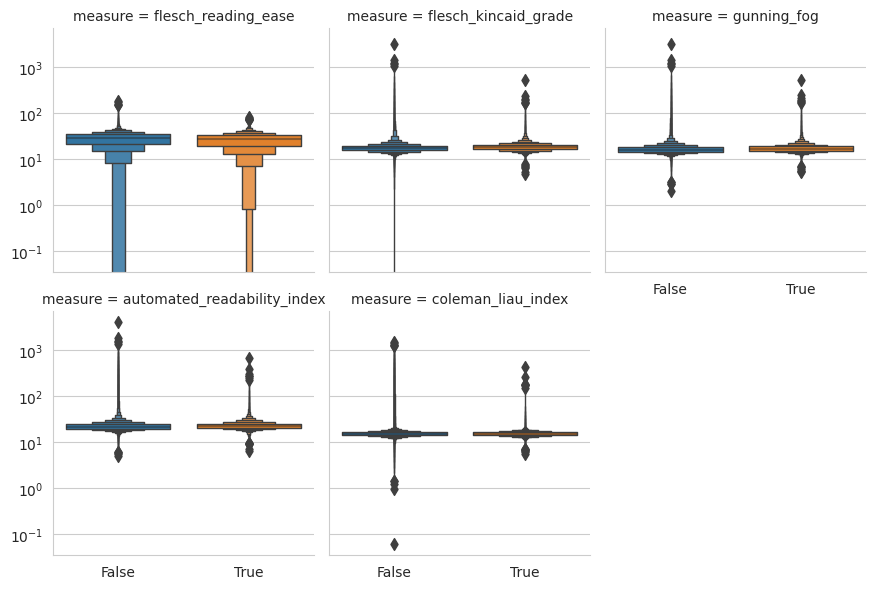
\includegraphics[width=8cm]{images/pmc.textstat.eng.boxplot.png}
    \caption{Traditional readability scores for English affiliation group (FAEA; n = 70,254)  and non-English affiliation group (FANA; n = 1,112,841)}
    \label{fig:readability-scores}
\end{figure}

\paragraph{LDA Coherence:}  By contrast, we found a significant difference between FAEA (n = 173,758) and non-english affiliation group (n = 2,244,040) when we applied LDA for assessing coherence (t = 48, p < 0.001). A comparison can be seen in Figure \ref{fig:lda-scores}. 

\begin{figure}
    \centering
    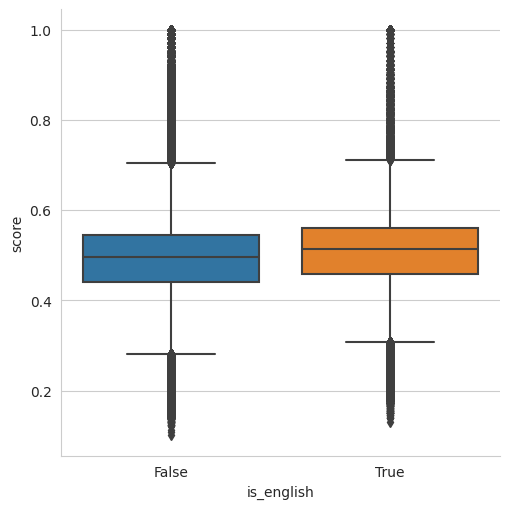
\includegraphics[width=8cm]{images/pmc.lda_coherence.score.boxplot.png}
    \caption{LDA coherence scores for English affiliation group (FAEA)  and non-English affiliation group (FANA)}
    \label{fig:lda-scores}
\end{figure}

This result is promising as it indicates that our LDA approach is able to measure differences in readability in scientific literature which cannot be reliably detected by traditional methods. However, this impact is mitigated by the effect of text length on LDA (Figure \ref{fig:lda-vs-text-size}). In the case of very short texts, we consistently obtained scores of 1.0, which is a spurious result. This reflects a limitation of LDA, namely that it does not perform well without sufficient text. Specifically, the topics in these samples are too sparse, given the choice of hyperparameters. This motivates our decision to exclude scores for short texts from our final LDA analysis.

\begin{figure}
    \centering
    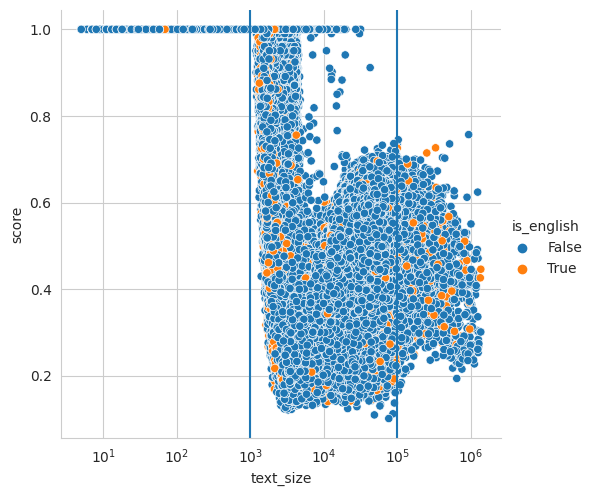
\includegraphics[width=8cm]{images/pmc.lda_coherence.text_size.scatter.png}
    \caption{The impact of text size (characters) on LDA scoring. Vertical lines show length thresholds of 1000 and 100000.}
    \label{fig:lda-vs-text-size}
\end{figure}

\paragraph{Concept Extraction:} 
Model training reproduced results reported in Brack et. al (Figure S\ref{fig:scibert-training-overall}). We achieved an f1-score of 0.67 on the validation set.
When applied to the PMC corpus, most concepts extracted (84\%, 7111604 of 8318150)  were unique to a single article (Figure \ref{fig:concepts-distribution}). 

\begin{figure}
    \centering
    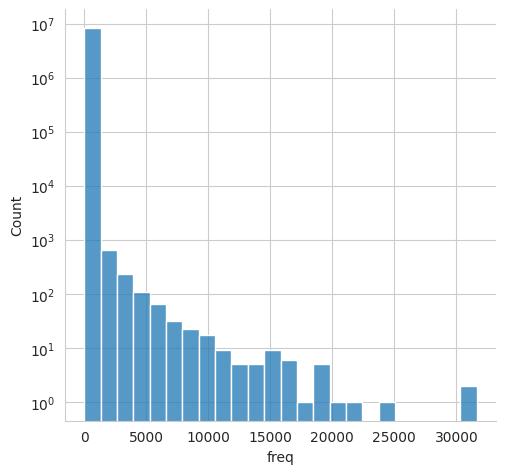
\includegraphics[width=8cm]{images/pmc.concepts.dist.png}
    \caption{Distribution of Extracted Scientific Concepts Shared amongst articles. }
    \label{fig:concepts-distribution}
\end{figure}

The extracted concepts were used to generate clusters of articles using agglomerative hierarchical clustering. Given that journals generally cover a single domain of science we expect articles within a journal to cover concepts more similar to other articles within that journal than articles outside the journal. The clustering result in Figure  \ref{fig:concept-cluster-composition} is consistent with this. Most clusters were relatively small (less than 100 articles) and composed of articles from a single journal (Figure \ref{fig:concept-cluster-composition}). 

\begin{figure}
    \centering
    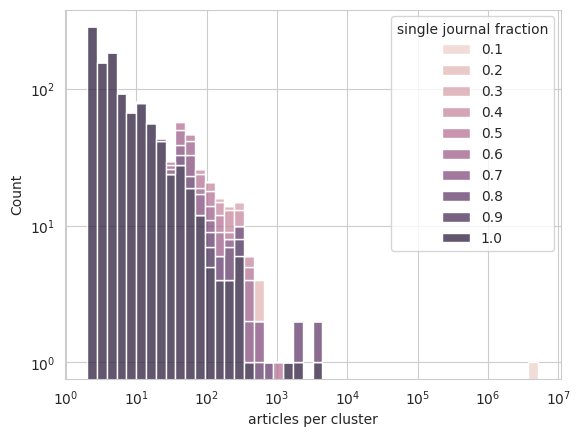
\includegraphics[width=8cm]{images/pmc.concepts.articles-per-cluster.png}
    \caption{Concept clusters of PMC articles based on concepts extracted using the domain in dependant extraction model. The x-axis shows the number of articles in each cluster. The y-axis shows the number of clusters with the given number of articles. The plot is colored by the maximum proportion of the articles in a given cluster which can be attributed to a single journal}
    \label{fig:concept-cluster-composition}
\end{figure}

In contrast, there was 1 large cluster which consisted of 28118 articles. Delving further into the contents of this cluster revealed that highly prevalent concepts (concepts present in more than 25\% of the articles included in the cluster) were very generic concepts such as: patient, increase, reduce, evaluate, treatment, decrease, assess, high, measure, analyze, effect, treat, and identify. \newline Future work could correct for this by using a similar method to TF-IDF but instead of word frequency using concept frequency. It is also likely that these represent higher levels of the hierarchical clustering and that introducing a maximum cluster size may have a similar effect.

\paragraph{Design of a System for Future Data Collection:}
A potential future area to explore is to collect data on how users browse scientific articles. The issue of readability of scientific texts for a research audience cannot be fully evaluated without further data. Thus, we propose an open-source browser extension (MyReads) to collect data on user behaviour when they access papers (Figure \ref{fig:chrome-ext}). 

\begin{figure*}
    \centering
    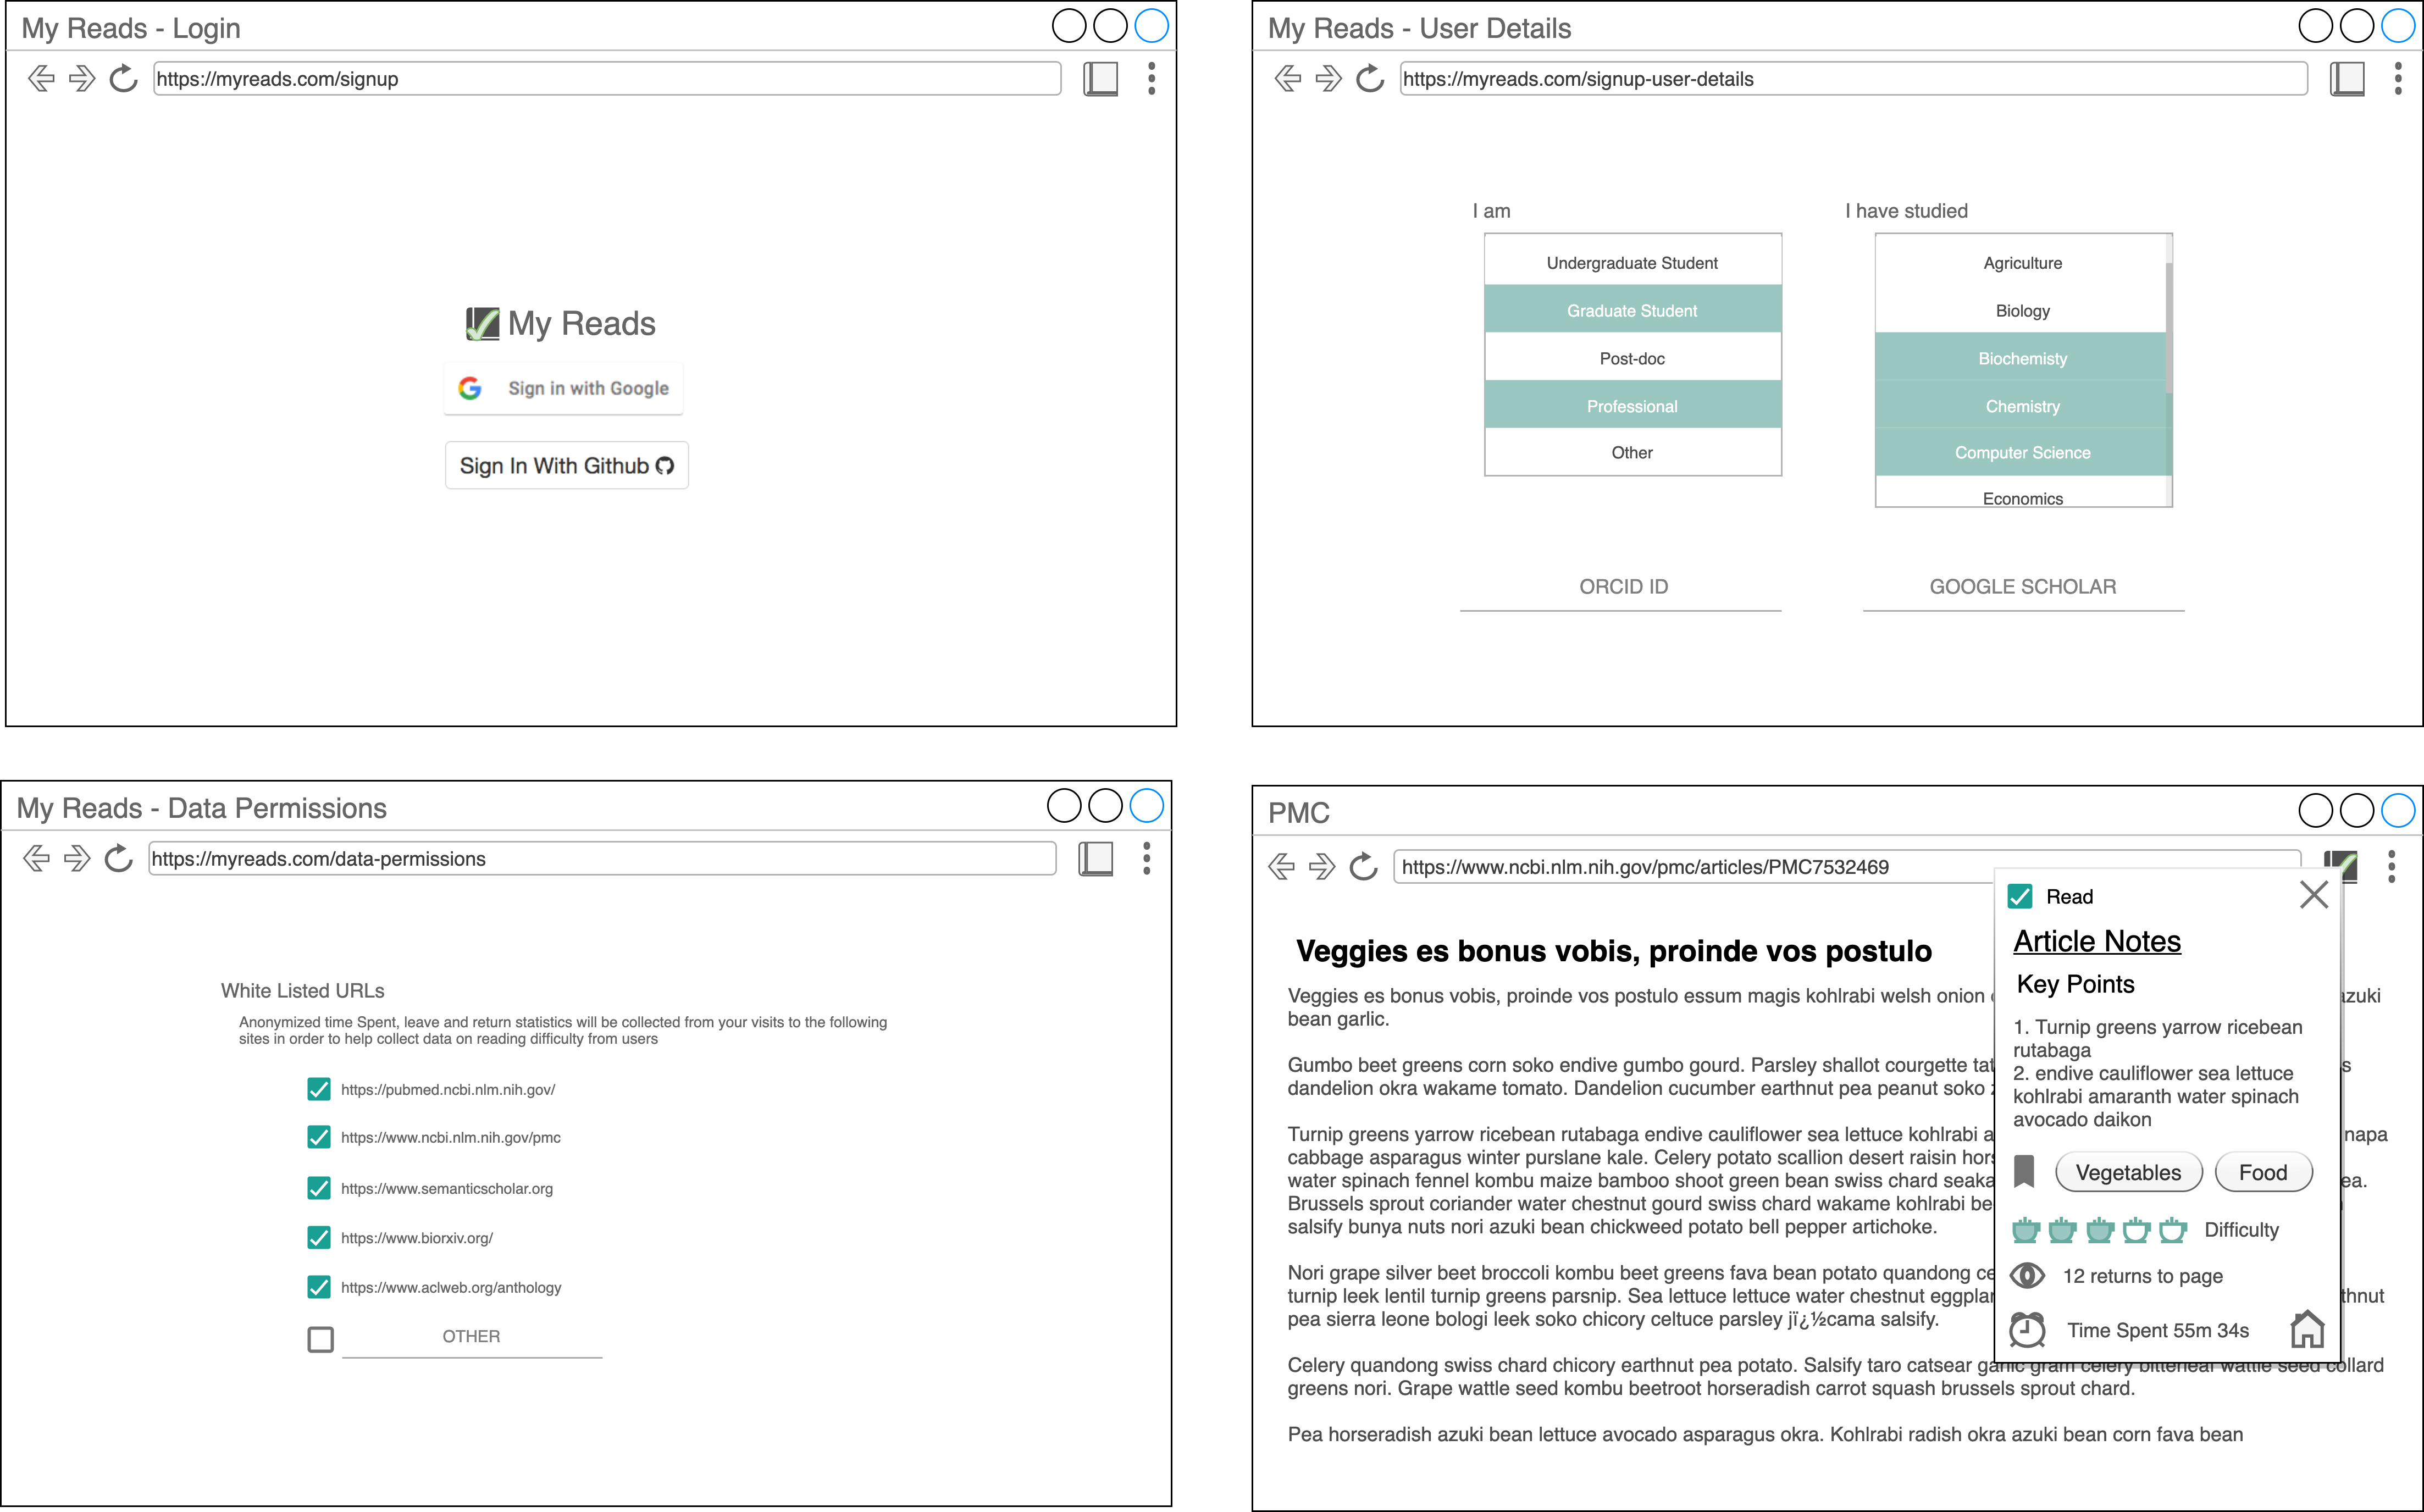
\includegraphics[width=15.5cm]{images/CPSC503-mockup-4-panel.png}
    \caption{Chrome Extension “MyReads”. Login or Sign up view (top left). New User background questions (top-right). User control of data collection (bottom left) and view of an article/URL the user has marked as read (bottom right). Automated data is collected on the time spent and number of times the user has left and re-focused the page as well as survey data representing the perceived difficulty. Options to tag and add notes are added for the convenience of the user.}
    \label{fig:chrome-ext}
\end{figure*}

The expected audience for the tool would be undergraduate and graduate students. The tool would measure time spent on a URL that is added and allow the user to add free text comments. The extension will user OpenAuth to allow users to easily login without storing passwords and other sensitive data (Figure \ref{fig:chrome-ext}). Following sign up the user will be directed to some initial survey questions which are designed to measure the starting background level of the user. These would include education level as well as areas of expertise. This data will allow us to account for the added difficulty of reading outside a users familiar discipline. In addition to passively collecting data on time-spent and returns to page as proxies for actual difficulty we will include an optional survey question with each article which will allow the user to record their perceived difficulty using a 5-point likert scale.

\section{Discussion}
\label{ssec:Discussion}

One limitation of our approach for converting articles to plain text was that we included all content, including formulas, citations, and figure captions. This introduced noise in the calculations. However, considering the size of the data set, the effect of this noise was smoothed out and it had a negligible impact on the results. 

Considering our LDA coherence calculation, we determined that text length is a confounding variable. However, it may be possible to compensate for text length to observe only differences due to variability in textual cohesion. For example, by tuning the LDA hyperparameters, it may be possible to mitigate this effect. Further work is needed to determine whether LDA could be effectively used to detect coherence between groups with variable-length texts.

Furthermore, we would like to explore other neural approaches for readability classification. Although this proved to be infeasible within the scope of this project, it would be useful to apply an RST-based classification approach, such as the one proposed by Guz et al. to the PMC data set. This would provide an informative comparison for assessing the effectiveness of our LDA-based model.

Time constraints preempted further analysis of the extracted concepts. In future work we would like to explore this with respect to the citation graph instead of only looking at journal level clustering.

Near-term future work should focus on the implementation of the data collection system we have described above (Figure \ref{fig:chrome-ext}), this will enable the collection of 'ground-truth' metrics without which any readability system will not be able to be fully evaluated. As the tool will allow students to organize their research and improve retention of readings, we expect this will be sufficient to motivate usage. We will use an opt-out consent model for the data collection. Once there are enough users for the data to be considered anonymous, we propose making open releases of the data set so that it may be used in future work.


\section{Conclusion}
\label{ssec:Conclusion}
\paragraph{}
In this project, we have applied existing methods for both readability scoring and concept extraction to scientific literature across a number of large scientific data sets, most notably PMC. We achieved a significant improvement in readability classification using LDA compared to traditional metrics. We also effectively trained and applied the Sci-BERT model to the concept extraction task. Ultimately, these methods are applicable in several areas, notably recommender systems for researchers. 
In both readability and concept extraction, we noted several remaining areas left to be investigated further. We would like to  explore the effect of document length on readability classification. Furthermore, we would like to assess the effectiveness of RST-based classification on our data. Finally, we proposed the design for an open-source system for future data collection which will be widely applicable in future studies.


\bibliography{acl2020}
\bibliographystyle{acl_natbib}


\clearpage



\section{Supplemental Material}
\label{sec:supplemental}
\textbf{Source Code:} All source code can be found in our GitHub repository at \url{https://github.com/creisle/cpsc503_final_project} 
Instructions are provided in the included README.md file. \newline


\noindent\textbf{Corpora:}\\* 
	-\href{https://www.ncbi.nlm.nih.gov/pmc/tools/openftlist/}{PMC}\\*
	-\href{https://github.com/aylai/GCDC-corpus}{GCDC}\\*
	-\href{https://github.com/elsevierlabs/OA-STM-Corpus}{OA-STM}\newline


\begin{figure}[ht]
    \centering
    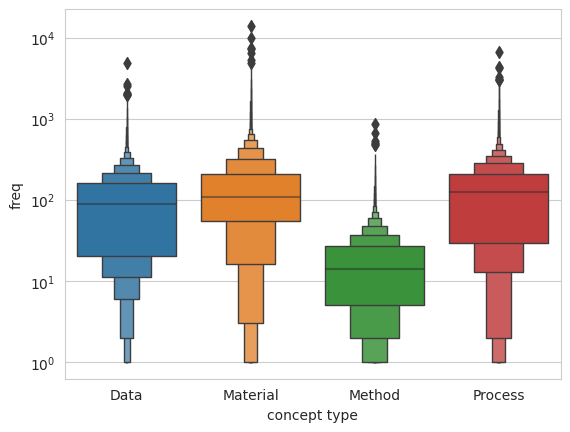
\includegraphics[width=8cm]{images/pmc.concepts.type_per_article.png}
    \caption{Average Number of Each Concept Type Extracted per Article}
    \label{fig:scibert-concept-types-per-article}
\end{figure}

\begin{figure*}
    \centering
    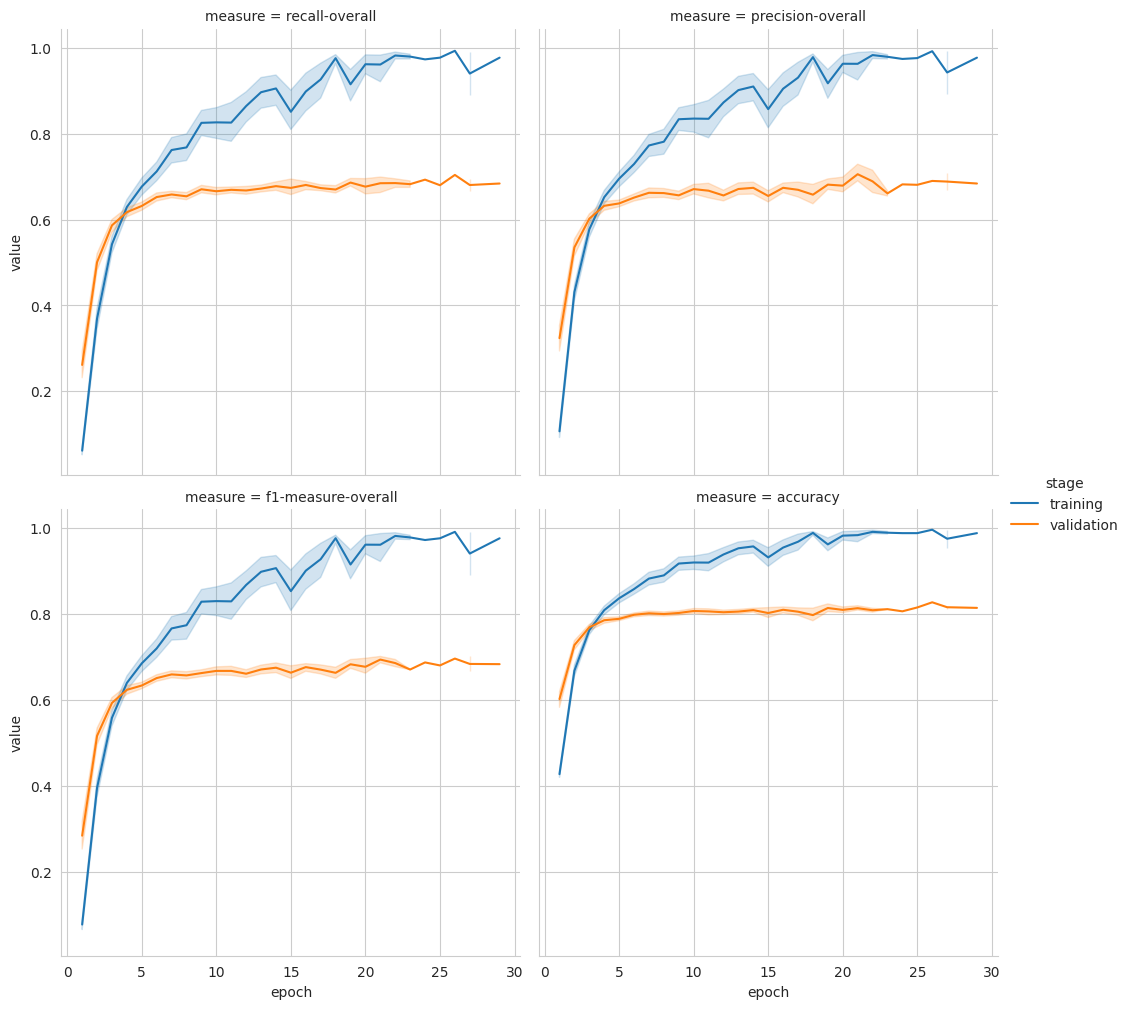
\includegraphics[width=15.5cm]{images/scibert.training_log.overall.png}
    \caption{Recall (top-left), Precision (top-right); F1 score (bottom left) and Accuracy (bottom right) by epoch during training of the domain independent concept extraction model on both the training and validation sets}
    \label{fig:scibert-training-overall}
\end{figure*}




\end{document}
